% 图序列化过程示意图 - 2×2 TikZ 布局
% Compile: xelatex seq_graph_tikz.tex  (在 drafts/figures/ 目录下)
\documentclass[tikz, border=8pt]{standalone}
\usepackage{tikz}
\usepackage{graphicx}
\usetikzlibrary{positioning, arrows.meta}

\begin{document}
\begin{tikzpicture}[
  imgw/.style={width=7.5cm},
  lbl/.style={
    text width=7.5cm, align=center,
    font=\small\ttfamily, text=#1
  },
  arr/.style={-{Stealth[length=12pt,width=8pt]}, line width=2.5pt, color=gray!60}
]

% ── 布局：上排 img1(左) img2(右)，下排 img4(左) img3(右)
% ── 箭头：1→2，2↓折→3，3←4
\node (img1) {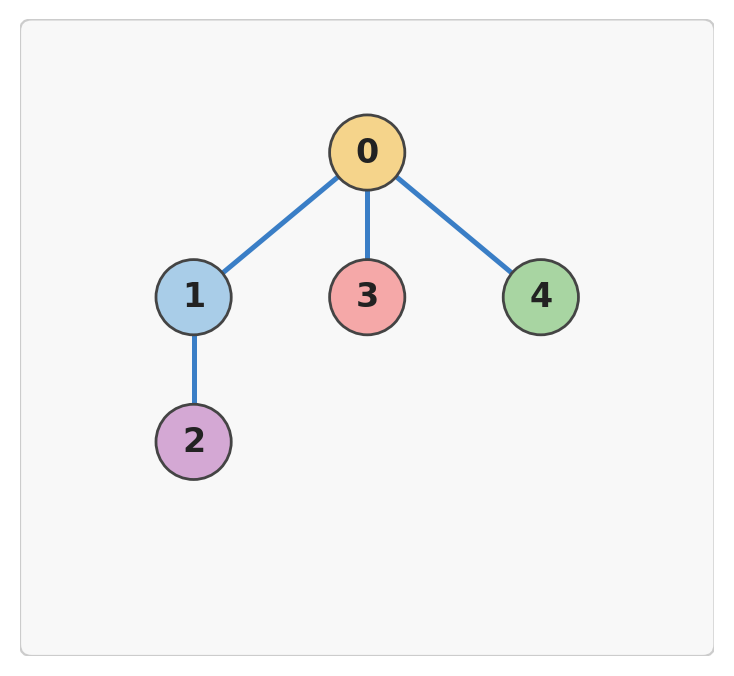
\includegraphics[width=7.5cm]{seq_graph_1.png}};
\node (img2) [right=1.6cm of img1] {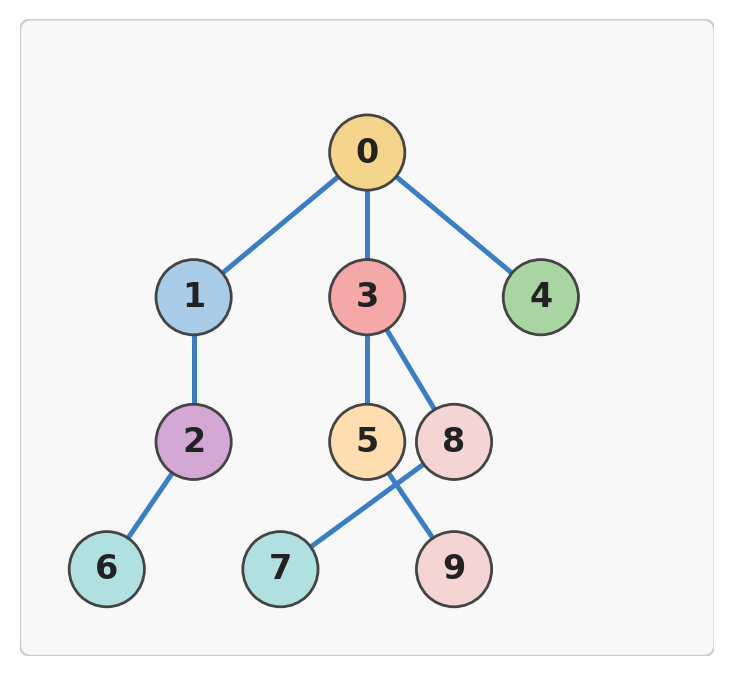
\includegraphics[width=7.5cm]{seq_graph_2.png}};
\node (img4) [below=2.2cm of img1] {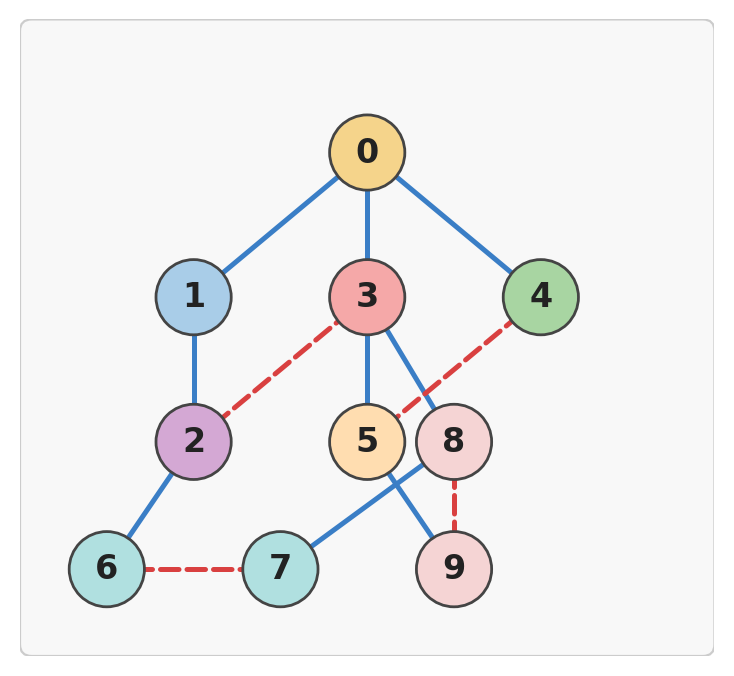
\includegraphics[width=7.5cm]{seq_graph_4.png}};
\node (img3) [right=1.6cm of img4] {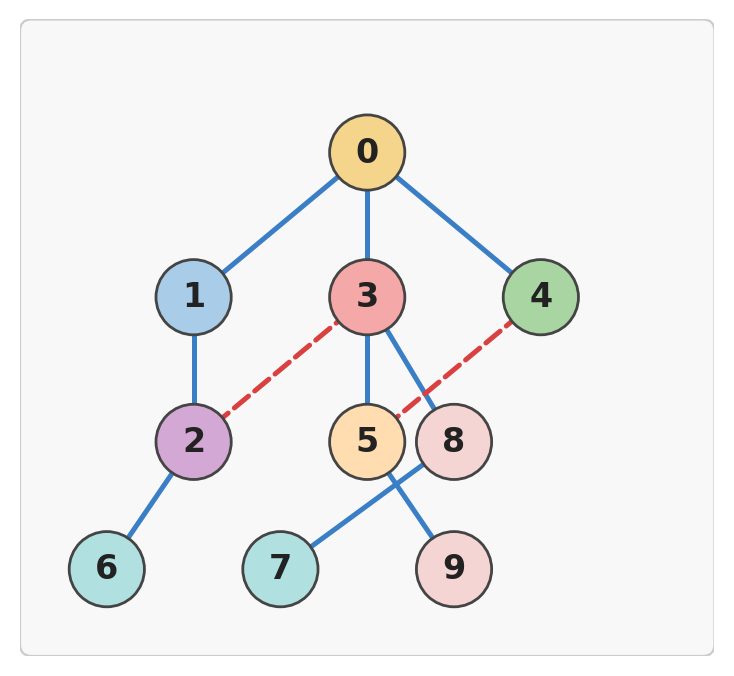
\includegraphics[width=7.5cm]{seq_graph_3.png}};

% ── token 序列（每张图下方）────────────────────────────────────────────────────
\node[lbl=black!80, below=0.25cm of img1.south] (tok1) {%
  BOS\_G\ \ $N_{10}$\ \ NODE$_0$\ \ NODE$_0$\ \ NODE$_0$\ \ NODE$_1$};

\node[lbl=black!80, below=0.25cm of img2.south] (tok2) {%
  BOS\_G\ \ $N_{10}$\ \ NODE$_0$\ \ NODE$_0$\ \ NODE$_0$\ \ NODE$_1$\\
  NODE$_3$\ \ NODE$_3$\ \ NODE$_2$\ \ NODE$_5$\ \ NODE$_8$\ \ SEP};

\node[lbl=black!80, below=0.25cm of img3.south] (tok3) {%
  BOS\_G\ \ $N_{10}$\ \ NODE$_0$\ \ NODE$_0$\ \ NODE$_0$\ \ NODE$_1$\\
  NODE$_3$\ \ NODE$_3$\ \ NODE$_2$\ \ NODE$_5$\ \ NODE$_8$\ \ SEP\\
  NODE$_2$\ \ NODE$_3$\ \ NODE$_4$\ \ NODE$_5$};

\node[lbl=black!80, below=0.25cm of img4.south] (tok4) {%
  BOS\_G\ \ $N_{10}$\ \ NODE$_0$\ \ NODE$_0$\ \ NODE$_0$\ \ NODE$_1$\\
  NODE$_3$\ \ NODE$_3$\ \ NODE$_2$\ \ NODE$_5$\ \ NODE$_8$\ \ SEP\\
  NODE$_2$\ \ NODE$_3$\ \ NODE$_4$\ \ NODE$_5$\ \ NODE$_6$\ \ NODE$_7$\\
  NODE$_8$\ \ NODE$_9$\ \ EOS\_G};

% ── 小标题（每张图上方）────────────────────────────────────────────────────────
\node[font=\normalsize\bfseries, above=0.18cm of img1.north] {(1) Partial spanning tree};
\node[font=\normalsize\bfseries, above=0.18cm of img2.north] {(2) Full spanning tree};
\node[font=\normalsize\bfseries, above=0.18cm of img3.north] {(3) Extra edges (partial)};
\node[font=\normalsize\bfseries, above=0.18cm of img4.north] {(4) Complete graph};

% ── 箭头：1→2（上排），2↓折→3（右侧），3←4（下排从右到左）─────────────────
\draw[arr] (img1.east) -- (img2.west);
\draw[arr] (img2.east) -- ([xshift=0.6cm]img2.east)
                       -- ([xshift=0.6cm]img3.east)
                       -- (img3.east);
\draw[arr] (img3.west) -- (img4.east);

\end{tikzpicture}
\end{document}
